\section{Buffer Amplifier}

Figure~\ref{BuffAmp} shows the schematic of the Buffer amplifier

\begin{figure}[h!]
  \centering
  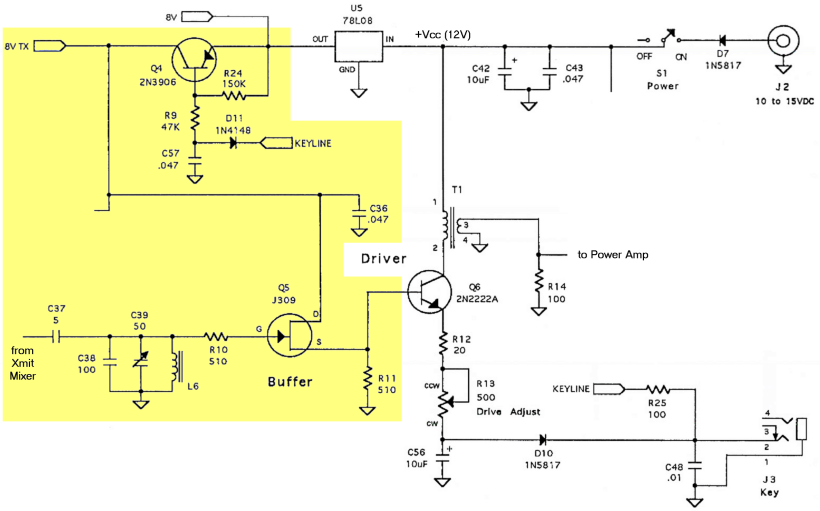
\includegraphics[scale=0.5]{./img/BuffAmp.png}
  \label{BuffAmp}
  \caption{Circuit Schematic for the Buffer Amplifier}
\end{figure}

Such a circuit is a source-follower, and therefore has no impedance gain and a
high input impedance. The function generator was connected to $C_{37}$ with
the $1.5k\Omega$ resistor. The frequency used was $7.04V$ and the amplitude
was $1V_{pp}$.

\subsection{Max Voltage Across \bm{$R_{10}$}}
$C_{39}$ was adjusted for maximum voltage. The measured maximum value
was $\boxed{ V}$.

\subsection{Voltage Gain across \bm{$R_{11}$}}
The voltage gain was measured to be $\boxed{ dB}$.

\subsection{Power Gain}
Given that a $1.5k\Omega$ resistor is at the input and a $510\Omega$ is
at the load, the power gain was calculated to be $\boxed{ dB}$
